%%%%%%%%%%%%%%%%%%%%%%%%%%%%%%%%%%%%%%%%%
% Beamer Presentation
% LaTeX Template
% Version 1.0 (10/11/12)
%
% This template has been downloaded from:
% http://www.LaTeXTemplates.com
%
% License:
% CC BY-NC-SA 3.0 (http://creativecommons.org/licenses/by-nc-sa/3.0/)
%
%%%%%%%%%%%%%%%%%%%%%%%%%%%%%%%%%%%%%%%%%

%----------------------------------------------------------------------------------------
%	PACKAGES AND THEMES
%----------------------------------------------------------------------------------------

\documentclass{beamer}
\mode<presentation> {

% The Beamer class comes with a number of default slide themes
% which change the colors and layouts of slides. Below this is a list
% of all the themes, uncomment each in turn to see what they look like.
%\usefonttheme{serif} % default family is serif
%\usefonttheme[onlymath]{serif}

%\usetheme{default}
%\usetheme{AnnArbor}
%\usetheme{Antibes}
%\usetheme{Bergen}
%\usetheme{Berkeley}
%\usetheme{Berlin}
%\usetheme{Boadilla} %Good choice
%\usetheme{CambridgeUS} %Good choice
%\usetheme{Copenhagen}
%\usetheme{Darmstadt}
%\usetheme{Dresden}
%\usetheme{Frankfurt}
%\usetheme{Goettingen}
%\usetheme{Hannover}
%\usetheme{Ilmenau}
%\usetheme{JuanLesPins}
%\usetheme{Luebeck}
\usetheme{Madrid} %Good choice
%\usetheme{Malmoe}
%\usetheme{Marburg}
%\usetheme{Montpellier}
%\usetheme{PaloAlto}
%\usetheme{Pittsburgh}
%\usetheme{Rochester}
%\usetheme{Singapore}
%\usetheme{Szeged}
%\usetheme{Warsaw} %Good choice

% As well as themes, the Beamer class has a number of color themes
% for any slide theme. Uncomment each of these in turn to see how it
% changes the colors of your current slide theme.

%\usecolortheme{albatross}
%\usecolortheme{beaver}
%\usecolortheme{beetle}
%\usecolortheme{crane} 
%\usecolortheme{dolphin}
%\usecolortheme{dove}
%\usecolortheme{fly}
%\usecolortheme{lily}
%\usecolortheme{orchid}
%\usecolortheme{rose}
%\usecolortheme{seagull}
%\usecolortheme{seahorse} %Good choice
%\usecolortheme{whale}
%\usecolortheme{wolverine} %Good choice

%This part is not really crucial
%\useinnertheme{inmargin} %circles, rectanges, rounded, inmargin
%\useoutertheme{tree} %infolines, smoothbars, sidebar, split, tree

%\setbeamertemplate{footline} % To remove the footer line in all slides uncomment this line
%\setbeamertemplate{footline}[page number] % To replace the footer line in all slides with a simple slide count uncomment this line

\setbeamertemplate{navigation symbols}{} % To remove the navigation symbols from the bottom of all slides uncomment this line

%\setbeamertemplate{background canvas}[vertical shading][bottom=white,top=structure.fg!25]
}

\usepackage{geometry}
\usepackage{xcolor}
\usepackage{tikz}
\usetikzlibrary{arrows,shapes,chains}

%\usetikzlibrary{positioning, arrows.meta}

\usepackage{graphicx} % Allows including images
\usepackage{booktabs} % Allows the use of \toprule, \midrule and \bottomrule in tables
\setbeamercovered{transparent} %This will make the preceding point transparent 
\usefonttheme[onlymath]{serif}
\setbeamertemplate{caption}[numbered]
%\setbeamerfont{title}{family={\fontfamily{Times}}}

%----------------------------------------------------------------------------------------
%	TITLE PAGE
%----------------------------------------------------------------------------------------
\title[Smart House]{Smart House: Remote Light Control} % The short title appears at the bottom of every slide, the full title is only on the title page

\author{Group 7} % Your name
\institute[XJTLU] % Your institution as it will appear on the bottom of every slide, may be shorthand to save space
{ 
Xian Jiaotong-Liverpool University \\ % Your institution for the title page
\medskip
%\textit{toting@xjtlu.edu.cn} % Your email address
}
\date{May 15, 2019} % Date, can be changed to a custom date

\tikzset{
	flowblock/.style = {
		rectangle,
		align = center,
		minimum size = 6mm,
		rounded corners = 2mm,
		very thick,
		draw = black!50,
		top color = white,
		bottom color = blue!50!white!20,
	}
}

\begin{document}

\begin{frame}
\titlepage % Print the title page as the first slide
\end{frame}

\begin{frame}
\frametitle{Outline} % Table of contents slide, comment this block out to remove it
\tableofcontents % Throughout your presentation, if you choose to use \section{} and \subsection{} commands, these will automatically be printed on this slide as an overview of your presentation
\end{frame}


%----------------------------------------------------------------------------------------
%	PRESENTATION SLIDES
%----------------------------------------------------------------------------------------

%------------------------------------------------
%\section{Structure and Flow} % Sections can be created in order to organize your presentation into discrete blocks, all sections and subsections are automatically printed in the table of contents as an overview of the talk
%------------------------------------------------

%\subsection{Subsection Example} % A subsection can be created just before a set of slides with a common theme to further break down your presentation into chunks

%This part is to display Table of Contents before new section. 
\AtBeginSection[]
{
\begin{frame}{Table of Contents} 
\tableofcontents[currentsection]
\end{frame}
}

%------------------------------------------------
\section{Introduction}
%------------------------------------------------


\begin{frame}{Introduction}
\begin{itemize}
\item The need for connectivity and remote control
\item Internet of Things (IoT)
\item Smart house - time-efficient and convenient
\end{itemize}
\end{frame}

\begin{frame}{Introduction}
\begin{block}<1->{Software}
	\vspace{-1.5em}
	\begin{columns}
		\column{0.4\textwidth}
		\begin{itemize}[<2->]
			\item WeChat mini program
			\item Web server development
		\end{itemize} 			
		\column{0.6\textwidth} 	
		\visible<2->{
			\begin{figure}
				
\includegraphics[scale=0.15]{img/mini_program.png}
			\end{figure}	
		}
	\end{columns}	

\end{block}

\begin{block}<1->{Hardware}
	\vspace{-0.6em}
	\begin{columns}
		\column[3->]{0.6\textwidth}
		\begin{itemize}[<3->]
			\item Arduino and ESP8266 Wi-Fi module
			\item Digital magnetic sensor
			\item Three LED lights
		\end{itemize}
	\column[<3->]{0.4\textwidth}
	\visible<3->{
		\begin{figure}
			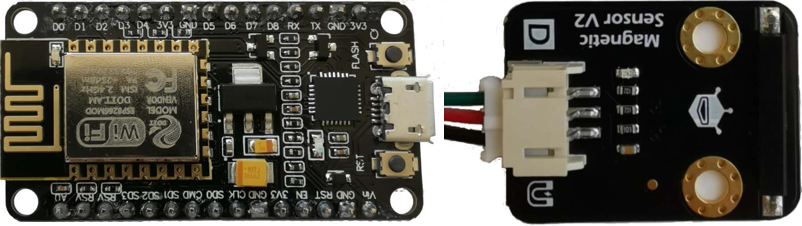
\includegraphics[scale=0.3]{img/equipment.png}
			\caption{Hardware equipment}
		\end{figure}
	}
	\end{columns}
	 
\end{block}
\end{frame}

%------------------------------------------------
\section{Methodology}
%------------------------------------------------
\begin{frame}{Methodology}
\begin{itemize}
	\item House model design
	\item Arduino design  
	\item Mini-program design
	\item Server design
\end{itemize}
\end{frame}

\begin{frame}{House model design}
\begin{columns}
	\column{0.6\textwidth}
	\begin{itemize}
		\item Living room - Red LED
		\item Bedroom - Yellow LED  
		\item Dining room - Green LED
		\item Single door - A digital magnetic sensor \\
		\qquad \qquad \quad- A magnet
	\end{itemize}
	\column{0.4\textwidth}
	\begin{figure}
		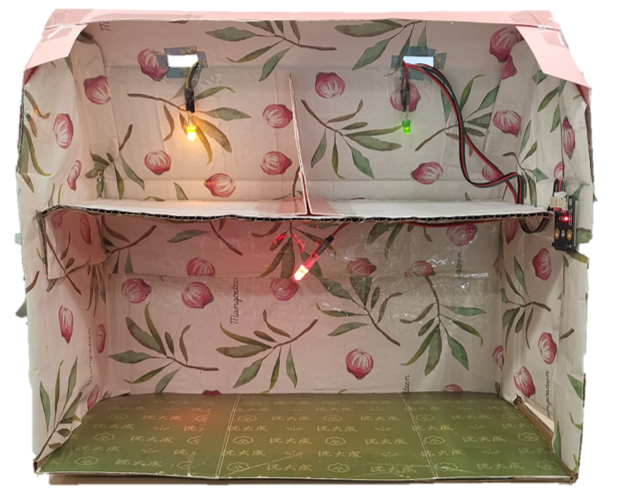
\includegraphics[scale=0.47]{img/house.png}
		\caption{House model}
	\end{figure}
	
\end{columns}

\end{frame}

\begin{frame}{Hosting Plan}
\begin{figure}
	\centering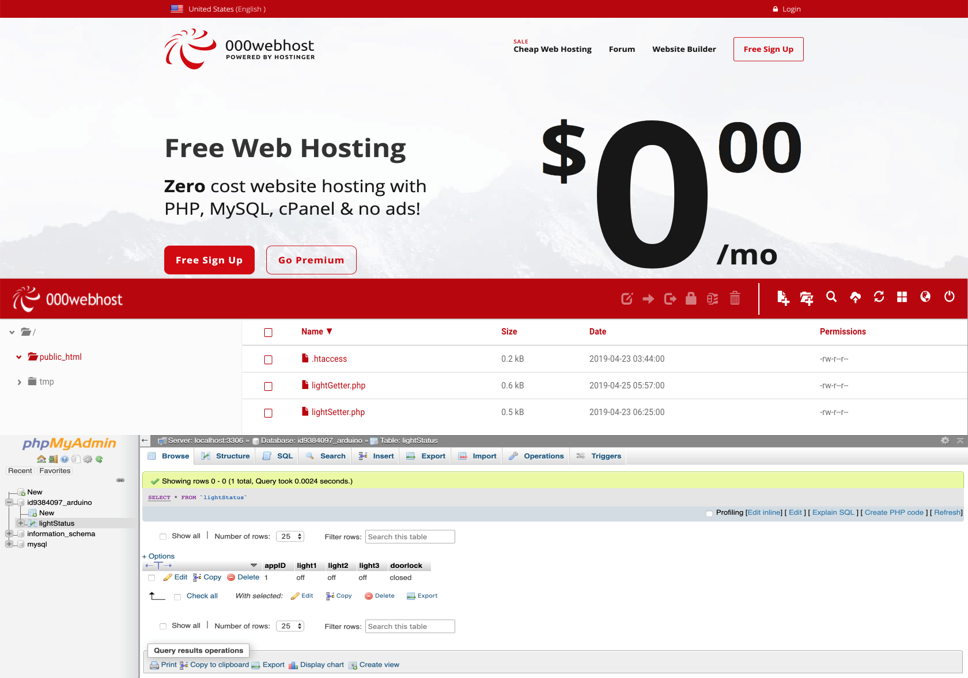
\includegraphics[width=12cm,height=7.5cm]{img/hosting_plan.png}
	%\caption{Hosting plan}
\end{figure}
\end{frame}

\begin{frame}{Processing Request}
\begin{figure}
	\centering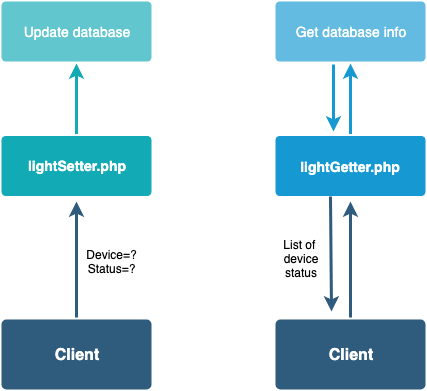
\includegraphics[width=9cm,height=7cm]{img/processing_requests.png}
	%\caption{processing requests}
\end{figure}
\end{frame}



\begin{frame}{Arduino Hardware}

\begin{block}<1->{Equipment}
\begin{itemize}
	\item ESP8266 $\rightarrow$ WiFi network
	\item Connected with UNO board $\rightarrow$ complicated
	\item NodeMCU = ESP8266 module + UNO board	
\end{itemize}
\end{block}

\begin{block}<2->{Circuit}
	\begin{columns}			
		\column{0.6\textwidth}
		\visible<2->{
			\begin{figure}
				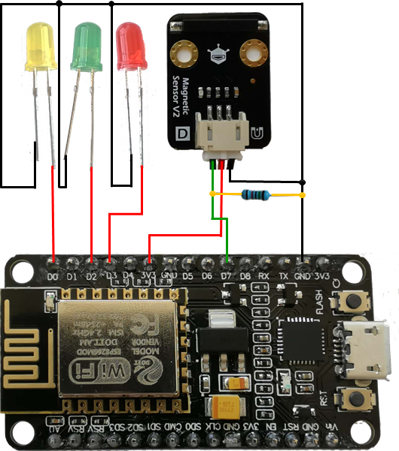
\includegraphics[scale=0.25]{img/circuit.png} 
				\caption{The whole circuit}
			\end{figure}
		}			
		\column{0.4\textwidth} 
		Resistor - Avoid Floating pin
	\end{columns}			

\end{block}
\end{frame}

\begin{frame}{Arduino Software}
\textbf{Two libraries}
\begin{enumerate}	
	\item<1-> \textbf{ESP8266WiFi.h} - connect to a given Wi-Fi network: router, hostspot
	\item<2-> \textbf{ESP8266HTTPClient.h} - send HTTP requests \\
	       \qquad \qquad \quad \ GET request - obtain each LED's status\\
	       \qquad \qquad \qquad \qquad \qquad \quad \ \ every 2s\\
	       \qquad \qquad \quad \ SET request - update the door's status
	       
\end{enumerate}
\end{frame}

\begin{frame}{WeChat Mini-Program UI}
\begin{figure}
	\centering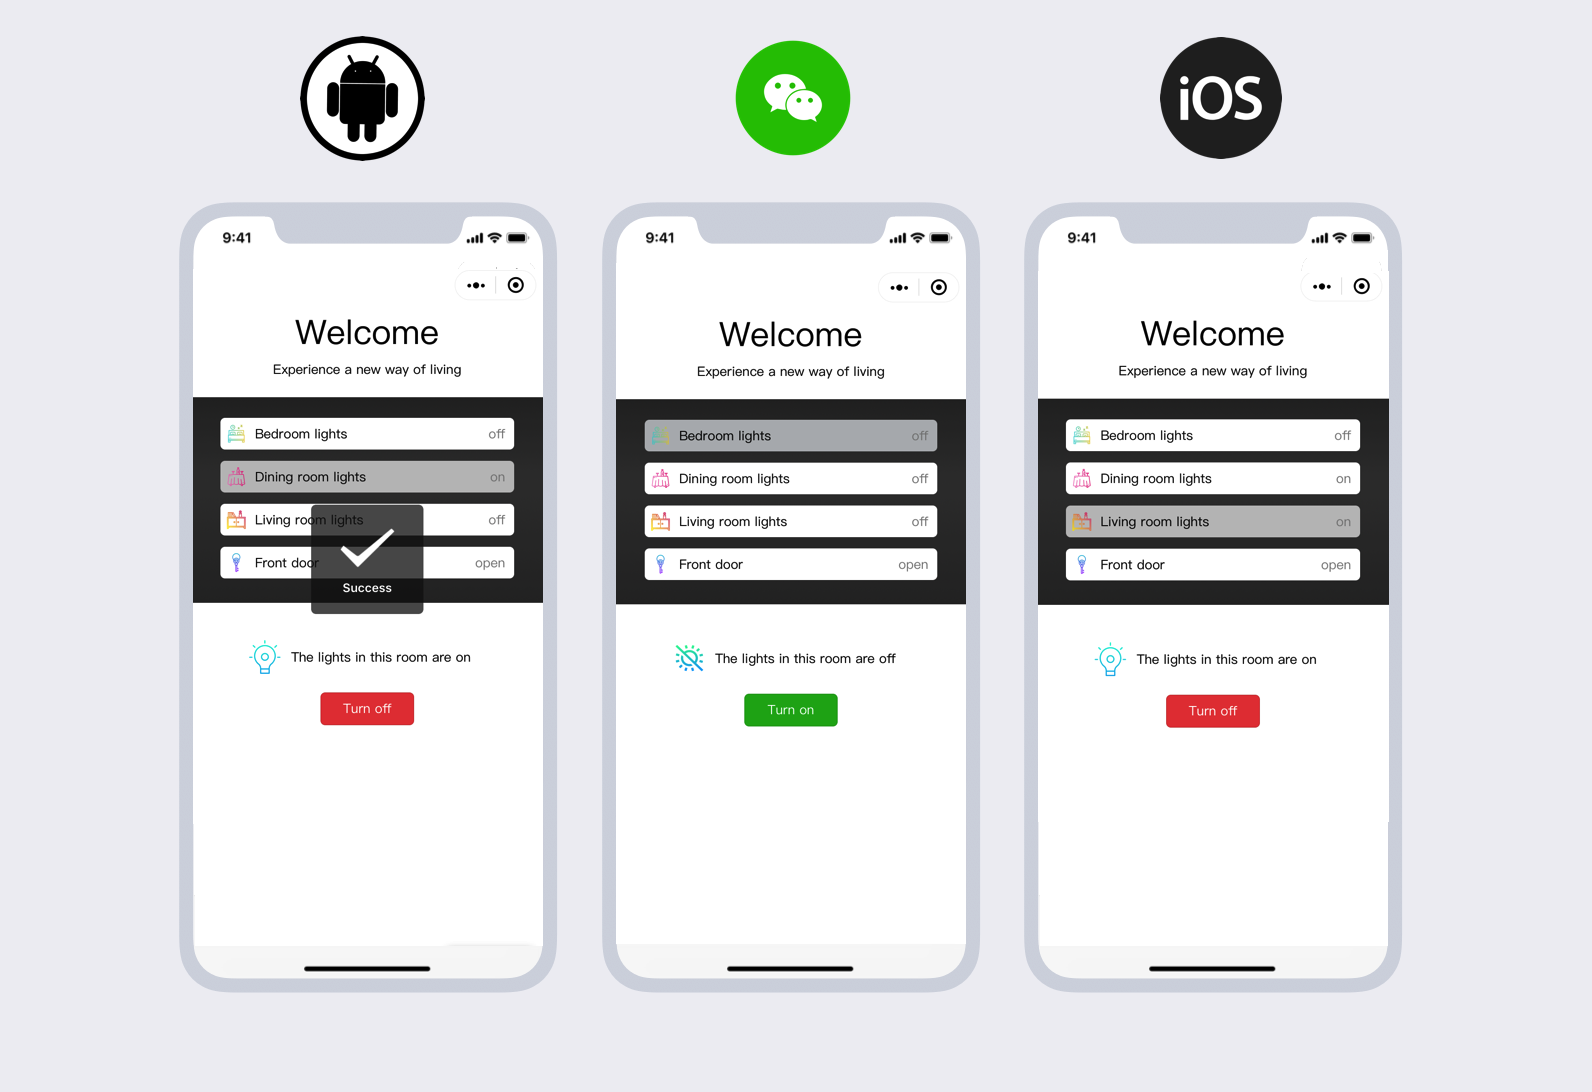
\includegraphics[width=12cm,height=8cm]{img/UI_2.png}
	%\caption{processing requests}
\end{figure}
\end{frame}

\begin{frame}{WeChat Mini-Program UI (cont.)}
\begin{figure}
	\centering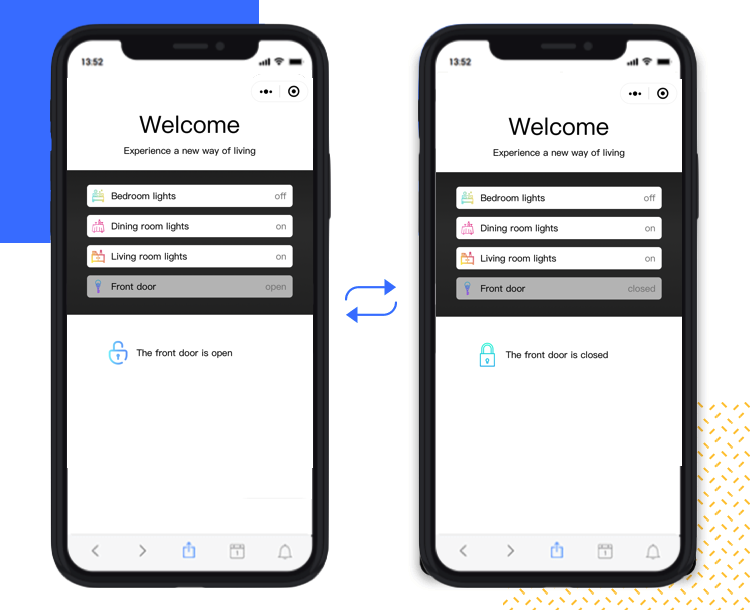
\includegraphics[width=12cm,height=8cm]{img/UI_con.png}
	%\caption{processing requests}
\end{figure}
\end{frame}

%------------------------------------------------
\section{Result}
%------------------------------------------------
\begin{frame}{Test}
\begin{itemize}
	\item<1-> Power supply - 5.1V / 2.1A\\
	          Network - personal hotspot	  
	\item<2-> Magnetic induction distance \\
		      1 magnet: 2mm $\sim$ 8mm $\xleftarrow[accurate]{more}$ Smart house model size\\
		      2 magnets: 10mm $\sim$ 22mm \\
	
	\item<3-> Testing by WeChat mini program 
	
\end{itemize}
\end{frame}

\begin{frame}{Result}
\textbf{Switch On / Off 3 LEDs}
	\begin{columns}			
	\column{0.4\textwidth}
	\begin{figure}
		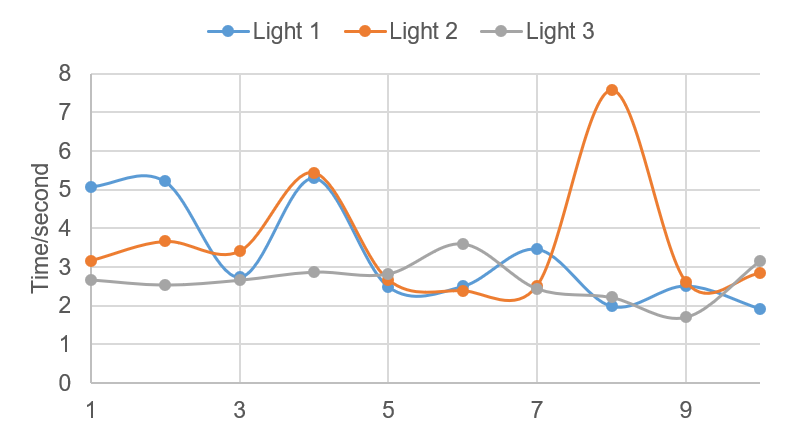
\includegraphics[width=5cm,height=4cm]{img/light_result.png} 
		\caption{Transmission time for change of light status}
	\end{figure}			
	\column{0.6\textwidth} 
	\begin{table}
		\centering
		\resizebox{5.5cm}{1cm}{
		\begin{tabular}{l l l l}
			\toprule
			 & \textbf{Bedroom} & \textbf{Dining room} & \textbf{Living room}\\
			\midrule
			$\bar{t}(s)$ & 3.322 & 3.631 & 2.670 \\
			Accuracy & \multicolumn{3}{l}{100 \%} \\
			\bottomrule
		\end{tabular}}
		\caption{Light transmission time}
	\end{table}
\end{columns}	

\end{frame}

\begin{frame}{Result}
\textbf{Check door statement}
\begin{columns}			
	\column{0.4\textwidth}
	\begin{figure}
		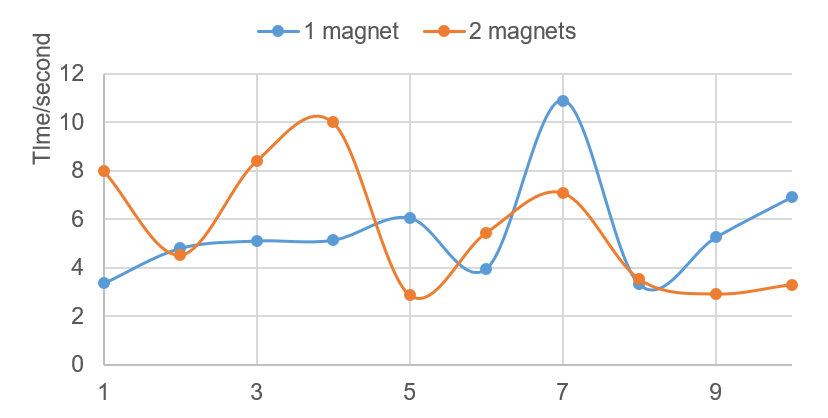
\includegraphics[width=5cm,height=4cm]{img/door_result.png} 
		\caption{Transmission time for change of door status}
	\end{figure}			
	\column{0.6\textwidth} 
	\begin{table}
		\begin{tabular}{l l l}
			\toprule
			\textbf{} & \textbf{1 magnet} & \textbf{2 magnets}\\
			\midrule
			$\bar{t}(s)$ & 5.481 & 5.687 \\
			Accuracy & \multicolumn{2}{l}{100 \%} \\
			\bottomrule
		\end{tabular}
		\caption{Door statement transmission time}
	\end{table}
\end{columns}	
\end{frame}






%------------------------------------------------
\section{Discussion}
%------------------------------------------------
\begin{frame}{Discussion}
\begin{itemize}
	\item Circuit design challenge
	\item Achievement 
	\item Problem
\end{itemize}
\end{frame}

\begin{frame}{Circuit design challenge}

	\textbf{Floating pin / Floating input:} affect the I/O pins of digital integrated circuits. \\
	\vspace{-1em}
	\begin{figure}
		\centering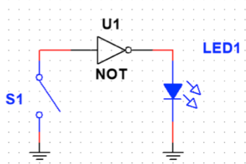
\includegraphics[scale=0.5]{img/floating_pin.png}
		\caption{Design causing Floating pin}
	\end{figure}

	\centering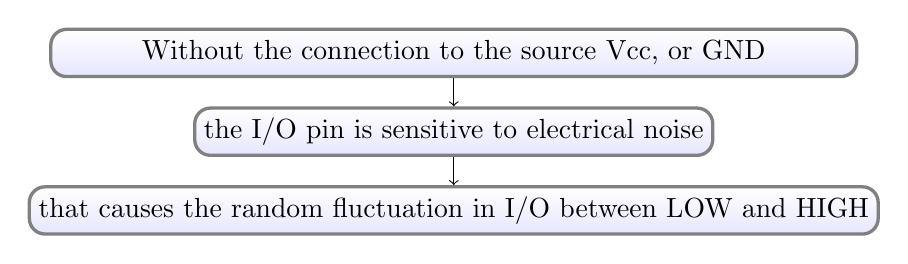
\begin{tikzpicture}[node distance = 1cm]
	\node[flowblock,text width = 10cm](upblock){Without the connection to the source Vcc, or GND};
	\node[flowblock, below of =  upblock](midblock){the I/O pin is sensitive to electrical noise};
	\node[flowblock, below of = midblock](bottom){that causes the random fluctuation in I/O between LOW and HIGH};
	
	\draw[->](upblock)--(midblock);
	\draw[->](midblock)--(bottom);
	\end{tikzpicture}

\end{frame}

\begin{frame}{Circuit design challenge}

\textbf{Solution}\\ The problem of ��floating pin�� can be solved by inserting a pull-up 15k��    lji resistor between I/O and GND.\\

\begin{figure}
	\centering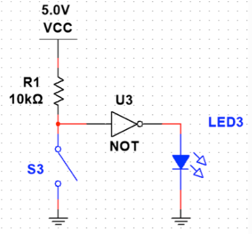
\includegraphics[scale=0.5]{img/floating_pin_design.png}
	\caption{The design for avoid Floating pin}
\end{figure}
\end{frame}

\begin{frame}{Achievement \& Problems}
\begin{block}<1->{Achievement}
\begin{itemize}
	\item Average time: within 5 seconds $\Rightarrow$ Response time is acceptable 
	\item Rate of failure  $\Rightarrow$ High rate of success 
\end{itemize}
\end{block}

\begin{block}<2->{Problems}
	\begin{itemize}
		\item Sometimes the response time have some delay
		\item Unstable fluctuation in response time
	\end{itemize}	
\end{block}

\end{frame}


%------------------------------------------------
\section{Future Work}
%------------------------------------------------

\begin{frame}{Future Work}
\textbf{5G}: enhance the transmission time and the possibility of failing will be decreased.\\
\begin{figure}
	\centering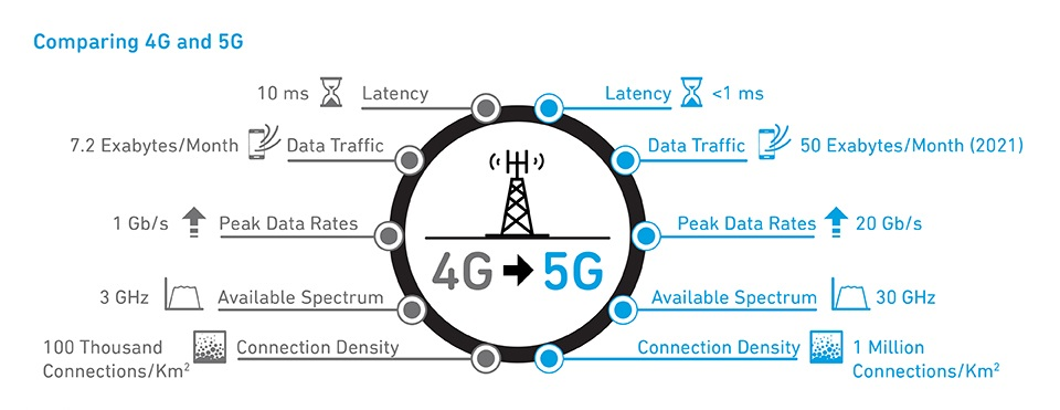
\includegraphics[width=12cm,height=5cm]{img/4G.png}
	\caption{Comparision of 4G and 5G}
\end{figure}
\end{frame}


\begin{frame}{Future Work}
	\begin{itemize}
	\item Use the server in local city
	\item Add more functions
	\item Security: verification and encryption protection - Hash codes	
	\end{itemize}
	\begin{columns}
		\column{0.4\textwidth}
		\begin{figure}
			
\includegraphics[scale=0.3]{img/server.png}
		\end{figure}
		\column{0.2\textwidth}
		\huge{\centerline{\textbf{+}}}
		\column{0.4\textwidth}
		\begin{figure}
			
\includegraphics[scale=0.3]{img/router.png}
		\end{figure}
	\end{columns}
\end{frame}
%------------------------------------------------

%----------------------------------------------------------------------------------------

\section{Conclusion}
%------------------------------------------------
% Citation
\begin{frame}{Conclusion}
\begin{itemize}
	\item Make a successful prototype
	\item Investigate IoT and hardware programming
	\item Improve teamworking and communication skills
\end{itemize}
\begin{figure}
	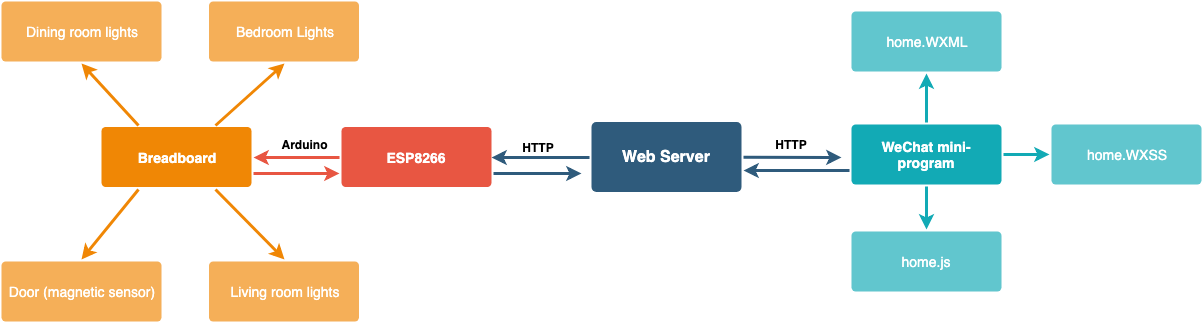
\includegraphics[width=11cm, height=4cm]{img/conclusion.png}
\end{figure}
\end{frame}

\begin{frame}
\Huge{\centerline{Question \& Answer}}
\end{frame}

\begin{frame}
\Huge{\centerline{Thank you}}
\end{frame}

\end{document} 